\documentclass[tikz, border=10pt]{standalone}
\usetikzlibrary{shapes,fit}

\tikzset{
    pics/vhsplit/.style n args = {2}{
        code = {
        \draw [draw] (0,1) rectangle (1.25,0.5);
        \node[draw=none] at (0.625,0.75) {#1};
        \draw [draw] (1.25,1) rectangle (2,0.5);
        \node[draw=none] at (1.625,0.75) {#2};
        \draw [draw] (0,0.5) rectangle (0.66,0);
        \draw [draw] (0.66,0.5) rectangle (1.32,0);
        \draw [draw] (1.32,0.5) rectangle (2,0);
        \node[draw=none] at (0.33,0.25) {\tiny{$<$}};
        \node[draw=none] at (1,0.25) {\tiny{$=$}};
        \node[draw=none] at (1.66,0.25) {\tiny{$>$}};
        }
    }
}


\begin{document}
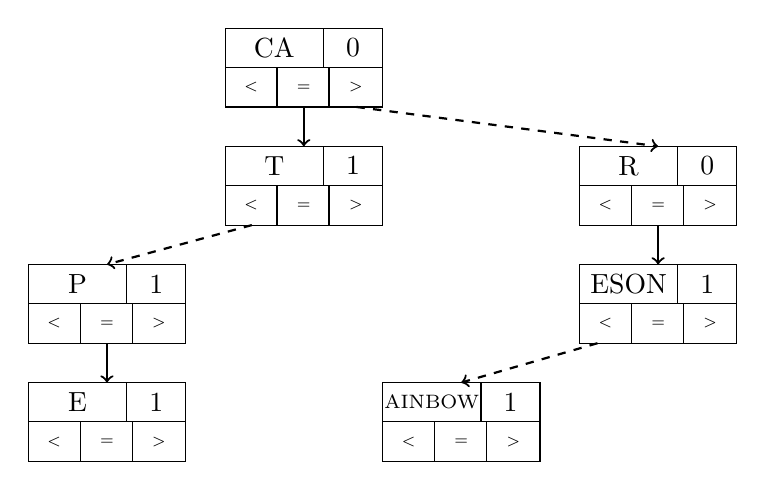
\begin{tikzpicture}%[every node/.append style={draw, rounded corners, inner sep=10pt}]
    \path pic at (-3,0) {vhsplit={CA}{0}};
    \coordinate(CAs) at (-2,0);
    \coordinate(Rs) at (-1.33,0);

    \path pic at (-3,-1.5) {vhsplit={T}{1}};
    \coordinate(CAn) at (-2,-0.5);
    \coordinate(Ts) at (-2.5,-1.5);
    \coordinate(Ps) at (-2.66,-1.5);

    \path pic at (-5.5,-3) {vhsplit={P}{1}};
    \coordinate(Pn) at (-4.5,-2);
    \coordinate(Es) at (-4.5,-3);

    \path pic at (-5.5,-4.5) {vhsplit={E}{1}};
    \coordinate(En) at (-4.5,-3.5);

    \draw [->,  thick] (CAs)--(CAn);
    \draw [->,  thick, dashed] (Ps)--(Pn);
    \draw [->,  thick] (Es)--(En);

    \path pic at (1.5,-1.5) {vhsplit={R}{0}};
    \coordinate(Rn) at (2.5,-0.5);
    \coordinate(E1s) at (2.5,-1.5);

    \path pic at (-1,-4.5) {vhsplit={\scriptsize{AINBOW}}{1}};
    \coordinate(A1n) at (0,-3.5);

    \path pic at (1.5,-3) {vhsplit={ESON}{1}};
    \coordinate(E1n) at (2.5,-2);
    \coordinate(A1s) at (1.73,-3);

    \draw [->,  thick, dashed] (Rs)--(Rn);
    \draw [->,  thick, dashed] (A1s)--(A1n);
    \draw [->,  thick] (E1s)--(E1n);

\end{tikzpicture}
\end{document}
